% ============================================================================
% Deep Surrogates to Estimate Dynamic Models
% Summer School on AI for Economics and Finance
% University of Padova, 23-24 September 2026
% Duration: 90 minutes
% ============================================================================

\documentclass[aspectratio=169,11pt]{beamer}

% ---------- Theme and colors ----------
\usecolortheme{dove}
\setbeamertemplate{navigation symbols}{}
\setbeamertemplate{footline}{%
  \hfill\usebeamerfont{page number in head/foot}%
  \usebeamercolor[fg]{normal text}%
  \insertframenumber\,/\,\inserttotalframenumber\kern1em\vskip4pt}
\setbeamerfont{frametitle}{size=\huge}

% ---------- Packages ----------
\usepackage[utf8]{inputenc}
\usepackage[T1]{fontenc}
\usepackage{amsmath,amssymb,amsfonts}
\usepackage{bm}
\usepackage{graphicx}
\usepackage{tikz}
\usetikzlibrary{shapes,arrows.meta,positioning,calc,fit,backgrounds,patterns,decorations.pathreplacing}
\usepackage{pgfplots}
\pgfplotsset{compat=1.18}
% --- readable-from-the-back defaults for every plot ---
\pgfplotsset{every axis/.append style={
    tick label style={font=\footnotesize},
    label style={font=\small},
    title style={font=\small},
    legend style={font=\footnotesize}}}
\usepgfplotslibrary{fillbetween}
\usepackage{booktabs}
\usepackage{hyperref}
\usepackage{multicol}
\usepackage{xcolor}
\usepackage{algorithmic}
\usepackage{listings}
\usepackage{pifont}
\usepackage{array}
\newcommand{\yes}{\textcolor{darkgreen}{\ding{51}}}
\newcommand{\no}{\textcolor{harvardcrimson}{\ding{55}}}
\newcommand{\mixed}{\textcolor{softorange}{\ding{108}}}

% ---------- Tighter display math, applied uniformly at every font size ------
% (a global typographic setting, so that no frame needs a local \vspace hack)
\makeatletter
\g@addto@macro\normalsize{%
  \setlength\abovedisplayskip{5pt plus 2pt minus 2pt}%
  \setlength\belowdisplayskip{5pt plus 2pt minus 2pt}%
  \setlength\abovedisplayshortskip{2pt plus 1pt}%
  \setlength\belowdisplayshortskip{3pt plus 1pt}}
\g@addto@macro\small{%
  \setlength\abovedisplayskip{4pt plus 2pt minus 2pt}%
  \setlength\belowdisplayskip{4pt plus 2pt minus 2pt}%
  \setlength\abovedisplayshortskip{2pt plus 1pt}%
  \setlength\belowdisplayshortskip{2pt plus 1pt}}
\g@addto@macro\footnotesize{%
  \setlength\abovedisplayskip{3pt plus 2pt minus 2pt}%
  \setlength\belowdisplayskip{3pt plus 2pt minus 2pt}%
  \setlength\abovedisplayshortskip{1pt plus 1pt}%
  \setlength\belowdisplayshortskip{2pt plus 1pt}}
\makeatother

% ---------- Custom colors ----------
\definecolor{uzhblue}{rgb}{0,0,0.5}
\definecolor{uzhgreylight}{RGB}{236,238,241}
\definecolor{uzhgreydark}{RGB}{81,86,94}
\definecolor{harvardcrimson}{RGB}{153,0,0}
\definecolor{unil@blue}{RGB}{0,140,204}
\definecolor{unil@black}{RGB}{35,31,32}
\definecolor{darkgreen}{RGB}{0,100,0}
\definecolor{darkred}{RGB}{139,0,0}
\definecolor{softblue}{RGB}{70,130,180}
\definecolor{softorange}{RGB}{230,159,0}
\definecolor{softgreen}{RGB}{0,158,115}

% ---------- Listings (after the colors it references) ----------
\lstset{
  language=Python,
  basicstyle=\small\ttfamily,
  keywordstyle=\color{uzhblue}\bfseries,
  commentstyle=\color{uzhgreydark}\itshape,
  stringstyle=\color{darkgreen},
  showstringspaces=false,
  breaklines=true,
  frame=none,
  aboveskip=2pt, belowskip=2pt}

% ---------- Set beamer colors ----------
\setbeamercolor{frametitle}{bg=uzhgreylight, fg=uzhblue}
\setbeamercolor{title}{fg=uzhblue}
\setbeamercolor{structure}{fg=uzhblue}
\setbeamercolor{block title}{bg=unil@blue, fg=white}
\setbeamercolor{block body}{bg=uzhgreylight}
\setbeamercolor{block title alerted}{bg=darkred,fg=white}
\setbeamercolor{block body alerted}{bg=red!5}
\setbeamercolor{block title example}{bg=darkgreen,fg=white}
\setbeamercolor{block body example}{bg=green!5}
\setbeamercolor{item}{fg=unil@black}
\setbeamercolor{normal text}{fg=unil@black}

% ---------- Emphasis and hyperlinks ----------
\newcommand{\emphc}[1]{\textcolor{harvardcrimson}{#1}}
\hypersetup{colorlinks,linkcolor=harvardcrimson,urlcolor=harvardcrimson}

% ---------- Finger-exercise badge ----------
\newcommand{\exercisepause}{%
  \tikz[baseline=(XB.base)]{%
    \node[rectangle, rounded corners=2pt, fill=softgreen!25, draw=softgreen!70!black,
          inner xsep=4pt, inner ysep=1.5pt,
          font=\footnotesize\bfseries, text=darkgreen] (XB) {PAUSE: 5 min};}}

% ---------- Math commands ----------
% One symbol, one meaning. See the notation frame in Part I.
% NOTE: this lecture is an estimation/policy lecture, so theta is the STRUCTURAL
% parameter vector, not the network weights (which the morning deck called theta).
\newcommand{\x}{\bm{x}}
\newcommand{\R}{\mathbb{R}}
\newcommand{\E}[1]{\mathbb{E}\!\left[#1\right]}
\newcommand{\str}{\bm{\theta}}          % structural parameters
\newcommand{\pol}{\bm{\vartheta}}       % policy parameters
\newcommand{\netw}{\bm{w}}              % network weights
\newcommand{\surr}{\phi}                % the surrogate
\DeclareMathOperator*{\argmin}{arg\,min}
\DeclareMathOperator*{\argmax}{arg\,max}

% ---------- Title ----------
\title[SMM -- Padova 2026]%
{Deep Learning for Solving Dynamic Models}
\subtitle{Session 7 --- Structural estimation via simulated method of moments}
\author{Simon Scheidegger}
\institute[HEC Lausanne]{HEC, University of Lausanne\\[4pt]
{\footnotesize Based on Chen, Didisheim \& Scheidegger (2026), \emph{Journal of Financial Economics} 177, 104222}}
\date{University of Padova\\September 24, 2026}

\begin{document}

% ============================================================================
% PART 0: TITLE & OUTLINE
% ============================================================================

% --- Slide 1: Title ---
{\setbeamercolor{background canvas}{bg=uzhgreylight}
\begin{frame}
\titlepage
\end{frame}
}

% --- Slide 2: Day 1 at a glance (same frame as lectures 1 and 2, marker moved) ---
\begin{frame}{Day 1 at a Glance}
\begin{center}
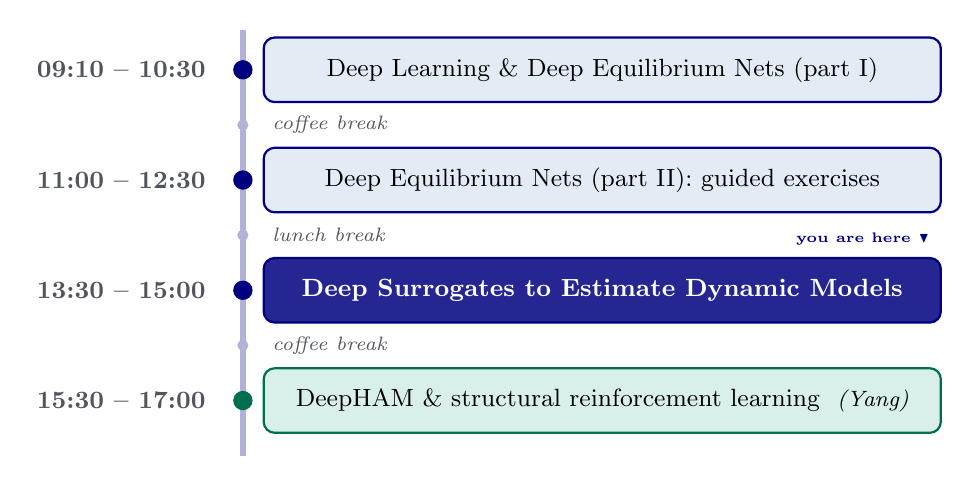
\begin{tikzpicture}[
    session/.style={rectangle, rounded corners=4pt, draw=uzhblue, thick, fill=softblue!15,
                    minimum width=8.6cm, minimum height=0.82cm, align=left, font=\small,
                    inner xsep=10pt, anchor=west},
    now/.style={session, fill=uzhblue!85, draw=uzhblue, text=white, font=\small\bfseries},
    guest/.style={session, fill=softgreen!15, draw=softgreen!70!black},
    pause/.style={font=\scriptsize\itshape, text=uzhgreydark, anchor=west},
    time/.style={font=\small\bfseries, text=uzhgreydark, anchor=east}
]
    \draw[uzhblue!30, line width=2pt] (0,0.5) -- (0,-4.9);

    \node[time] at (-0.35, 0) {09:10 -- 10:30};
    \node[session] at (0.25, 0) {Deep Learning \& Deep Equilibrium Nets (part I)};
    \fill[uzhblue] (0,0) circle (3.5pt);

    \node[pause] at (0.25,-0.7) {coffee break};
    \fill[uzhblue!30] (0,-0.7) circle (2pt);

    \node[time] at (-0.35,-1.4) {11:00 -- 12:30};
    \node[session] at (0.25,-1.4) {Deep Equilibrium Nets (part II): guided exercises};
    \fill[uzhblue] (0,-1.4) circle (3.5pt);

    \node[pause] at (0.25,-2.1) {lunch break};
    \fill[uzhblue!30] (0,-2.1) circle (2pt);

    \node[time] at (-0.35,-2.8) {13:30 -- 15:00};
    \node[now] at (0.25,-2.8) {Deep Surrogates to Estimate Dynamic Models};
    \fill[uzhblue] (0,-2.8) circle (3.5pt);
    \node[font=\tiny\bfseries, text=uzhblue, anchor=south east] at (8.85,-2.35) {you are here $\blacktriangledown$};

    \node[pause] at (0.25,-3.5) {coffee break};
    \fill[uzhblue!30] (0,-3.5) circle (2pt);

    \node[time] at (-0.35,-4.2) {15:30 -- 17:00};
    \node[guest] at (0.25,-4.2) {DeepHAM \& structural reinforcement learning~~{\footnotesize\itshape (Yang)}};
    \fill[softgreen!70!black] (0,-4.2) circle (3.5pt);
\end{tikzpicture}
\end{center}

\vspace{0.1cm}
\begin{center}
{\footnotesize \textbf{Materials:}~\href{https://github.com/sischei/deep_learning_padova_0926}{github.com/sischei/deep\_learning\_padova\_0926}~~$\cdot$~~\textbf{Cloud:}~\href{https://nuvolos.cloud}{nuvolos.cloud}}
\end{center}
\end{frame}

% --- Slide 3: Roadmap ---
\begin{frame}{Roadmap of This Lecture (90 min)}
\begin{columns}[T]
\column{0.48\textwidth}
\textbf{I.\ What Is a Surrogate?}~~\mbox{\small (12 min)}
\begin{itemize}\setlength\itemsep{1pt}
    \item Look-up tables, pseudo-states, and what the speed-up buys
\end{itemize}

\vspace{0.4em}
\textbf{II.\ Estimate:} structural estimation~~\mbox{\small (20 min)}
\begin{itemize}\setlength\itemsep{1pt}
    \item SMM on a surrogate; Brock--Mirman; the identification ridge
\end{itemize}

\vspace{0.4em}
\textbf{III.\ Gaussian Processes}~~\mbox{\small (24 min)}
\begin{itemize}\setlength\itemsep{1pt}
    \item When data is expensive, a deep net is the wrong tool
    \item Kernels, credible bands, and active learning
\end{itemize}

\column{0.48\textwidth}
\textbf{IV.\ Quantify:} uncertainty~~\mbox{\small (10 min)}
\begin{itemize}\setlength\itemsep{1pt}
    \item Univariate effects, Sobol' indices, Shapley values for the SCC
\end{itemize}

\vspace{0.4em}
\textbf{V.\ Design:} the optimal carbon tax~~\mbox{\small (16 min)}
\begin{itemize}\setlength\itemsep{1pt}
    \item Policy coefficients as pseudo-states; 500 solves, not a million
\end{itemize}

\vspace{0.4em}
\textbf{VI.\ Synthesis and Hands-On}~~\mbox{\small (8 min)}
\begin{itemize}\setlength\itemsep{1pt}
    \item When to use what; the notebooks
\end{itemize}
\end{columns}
\end{frame}

% --- Slide 4: Learning objectives ---
\begin{frame}{Learning Objectives}
\textbf{By the end of this lecture you should be able to:}
\begin{itemize}\itemsep3pt
  \item Explain a surrogate as a \emphc{differentiable look-up table} and say precisely which classical bottleneck it removes
  \item Promote structural or policy parameters to \emphc{pseudo-states}, so that one solve answers a whole family of questions
  \item Estimate a structural parameter by simulated method of moments on a trained surrogate, and read an identification ridge off the criterion surface
  \item Turn the same surrogate into a global sensitivity analysis: univariate effects, Sobol' indices, Shapley values
  \item Fit a Gaussian process, read its credible band, and \emphc{decide between a GP and a deep network} from the cost of one model evaluation
  \item Place the next expensive evaluation where it buys the most, using Bayesian active learning
\end{itemize}
\end{frame}

% ============================================================================
% PART I: WHAT IS A SURROGATE?
% ============================================================================

% --- Padova cut: section 1 "What Is a Surrogate?" (245 lines) dropped ---
\section{Estimate: Structural Estimation}

\begin{frame}{}
\begin{center}
{\Huge \textcolor{uzhblue}{Part II}}\\[0.8em]
{\LARGE Estimate: Structural Estimation}
\end{center}
\end{frame}

% --- The estimation loop ---
\begin{frame}{The Estimation Loop, and Why It Is Expensive}
\textbf{The classical nested fixed point.} For each candidate $\str$:
\begin{center}
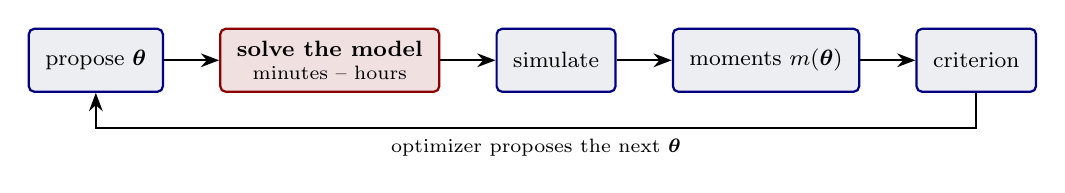
\begin{tikzpicture}[
    box/.style={rectangle, draw=uzhblue, thick, rounded corners=2pt, fill=uzhgreylight,
                minimum height=0.8cm, font=\footnotesize, align=center, inner xsep=6pt},
    >=Stealth
]
\node[box] (guess) {propose $\str$};
\node[box, right=0.7cm of guess, fill=darkred!12, draw=darkred] (solve) {\textbf{solve the model}\\[-1pt]{\scriptsize minutes -- hours}};
\node[box, right=0.7cm of solve] (sim) {simulate};
\node[box, right=0.7cm of sim] (mom) {moments $m(\str)$};
\node[box, right=0.7cm of mom] (crit) {criterion};
\draw[->, thick] (guess) -- (solve);
\draw[->, thick] (solve) -- (sim);
\draw[->, thick] (sim) -- (mom);
\draw[->, thick] (mom) -- (crit);
\draw[->, thick] (crit.south) -- ++(0,-0.45) -| node[pos=0.25, below, font=\scriptsize] {optimizer proposes the next $\str$} (guess.south);
\end{tikzpicture}
\end{center}

\vspace{0.5cm}
\textbf{The surrogate move.} Put $\str$ \emph{inside} the network at training time. The red box then runs \emphc{once}, and the loop becomes a forward pass.

\vspace{0.3cm}
\begin{block}{Two consequences, not one}
\begin{itemize}\itemsep1pt
  \item The criterion becomes cheap enough to evaluate on a fine grid, so you can \emph{look at} it rather than trust a local optimizer's report.
  \item The criterion becomes \emphc{differentiable in $\str$}, because the surrogate is.
\end{itemize}
\end{block}
\end{frame}

% --- SMM 1 ---
\begin{frame}{SMM: The Moment Condition}
\small
Let the data give $T$ observations $\{y_t\}$. Choose moment functions $g(y)\in\R^{q}$ such that, at the true parameter $\str_0 \in \R^{p}$ with $q \ge p$,
\[
\E{g(y_t) - m(\str_0)} = 0,
\qquad m(\str) = \mathbb{E}_{\str}[g(y_t)] .
\]
The empirical and simulated counterparts are
\[
\widehat g_T = \tfrac{1}{T}\sum_{t=1}^{T} g(y_t),
\qquad
\widehat m_S(\str) = \tfrac{1}{S}\sum_{s=1}^{S} g\bigl(y^{\mathrm{sim}}_s(\str)\bigr).
\]

\vspace{0.2em}
\textbf{Identification.} $\str_0$ is the \emph{unique} zero of $\E{g(y_t)} - m(\str)$ on the parameter space. Just-identified: $q = p$. Over-identified: $q > p$, which buys a testable restriction. It does \emph{not} automatically sharpen the criterion: a moment with a near-zero column in $M$ adds noise and finite-sample bias, as the joint exercise will show.

\vspace{0.2em}
\textbf{In this lecture.} $y_t$ is log output, consumption, and capital; $g$ collects three volatility and autocorrelation moments; $\str = \varrho$ first, then $\str = (\beta,\varrho)$.
\end{frame}

% --- SMM 2 ---
\begin{frame}{SMM: Estimator and Weighting}
\small
\[
\widehat{\str}_{\mathrm{SMM}} = \argmin_{\str}\;
\bigl[\widehat g_T - \widehat m_S(\str)\bigr]^{\!\top} W \bigl[\widehat g_T - \widehat m_S(\str)\bigr],
\qquad W \succ 0 .
\]

\vspace{0.3em}
\begin{alertblock}{Common random numbers: the detail that decides success}
Hold the shock draws $\{\varepsilon_s\}$ \emphc{fixed across $\str$}. Then $\widehat m_S(\str)$ is a smooth function of $\str$, with a clean minimum. Re-draw them and you are optimizing a noisy surface: the optimizer chases simulation noise and reports wherever it happened to land.
\end{alertblock}

\vspace{0.2em}
\textbf{Weighting matrix.}
\begin{itemize}\itemsep1pt
  \item \emphc{Identity} $W = I$: the honest pedagogical default; consistent, inefficient.
  \item \emphc{Diagonal} $W = \mathrm{diag}(1/\hat\sigma_g^2)$: rescales each moment by its sampling variance.
  \item \emphc{Optimal} $W^\star = \Omega^{-1}$, the inverse asymptotic covariance of the moment gap, proportional to $\widehat\Sigma_g^{-1}$ up to the simulation factor $1 + 1/S$. Minimum asymptotic variance. ($S = 10$ costs 5\% in standard errors; $S = 1$ costs 41\%.)
\end{itemize}
\end{frame}

% --- SMM 3 ---
\begin{frame}{SMM: What the Asymptotics Tell You to Look At}
\small
Write $M = \partial m(\str_0)/\partial\str^\top$ for the moment Jacobian, and $\Omega$ for the asymptotic covariance of the \emphc{moment gap} $\sqrt{T}\bigl[\widehat g_T - \widehat m_S(\str_0)\bigr]$. If the simulated shocks are drawn independently of the data, $\Omega = (1 + 1/S)\,\widehat\Sigma_g$ with $S$ panels of the data's length; as $S \to \infty$, $\Omega \to \widehat\Sigma_g$. \emphc{The inflation is the price of simulating rather than solving.}

\vspace{0.2em}
Under the usual regularity conditions, as $T \to \infty$,
\[
\sqrt{T}\,\bigl(\widehat{\str}_{\mathrm{SMM}} - \str_0\bigr) \;\xrightarrow{d}\; \mathcal{N}\bigl(0, V(W)\bigr),
\qquad
V(W) = (M^\top W M)^{-1} M^\top W \,\Omega\, W M (M^\top W M)^{-1},
\]
which collapses to $V(W^\star) = (M^\top \Omega^{-1} M)^{-1}$ at the efficient weighting.

\vspace{0.3em}
\begin{block}{Identification, read geometrically}
$V$ exists only if $M$ has \emphc{full column rank}. A near-rank-deficient $M$ is a \emphc{flat direction} of the criterion: an \emph{identification ridge}. Standard errors explode, the point estimate is arbitrary along the ridge, and no amount of data at those moments fixes it.

\vspace{2pt}
Because the surrogate makes the criterion cheap, you can \emphc{plot the ridge} instead of inferring it from an ill-conditioned Hessian. We do exactly that at the end of this part.
\end{block}
\end{frame}

% --- What the surrogate costs you, econometrically ---
\begin{frame}{The Surrogate Is Not Free}
\small
Everything on the previous slide assumed the moments came from \emph{the model}. They came from a network. Write $\widehat m = m + e$, where $e$ is the surrogate's approximation error.

\vspace{0.15cm}
\begin{alertblock}{$e$ does not shrink with the sample}
More data makes $\widehat g_T$ precise; it does nothing to $e$. This is \emphc{non-local misspecification}: the estimator converges not to $\str_0$ but to a \emphc{pseudo-true} $\str^\star$ minimizing the population criterion under $\widehat m$, with Hall--Inoue asymptotics rather than Hansen's.
\vspace{2pt}
\[
\sqrt{T}\bigl(\widehat{\str} - \emphc{\str^\star}\bigr) \;\xrightarrow{d}\; \mathcal{N}\bigl(0, \Sigma(\mu^\star)\bigr),
\qquad \str^\star \to \str_0 \ \text{ only as } \ \sup_{\str} \|e(\cdot,\str)\| \to 0 .
\]
\end{alertblock}

\vspace{0.1cm}
\textbf{The practical consequence}, and the whole reason Part I ended with a validation step: report the surrogate's \emphc{maximum} error over the parameter box, not its mean. The maximum bounds the bias, and a surrogate with excellent \emph{average} accuracy can still be badly wrong in the one direction you are estimating. That happens at the end of this part.

\vspace{0.05cm}
{\footnotesize Chen, Didisheim \& Scheidegger (2026), fn.\ 15, make the point about their own surrogate; the asymptotics are Hall \& Inoue (2003).}
\end{frame}

% --- The model ---
\begin{frame}{The Model: Brock--Mirman with Stochastic TFP}
\small
The same model class as this morning, with two deliberate changes: $\delta$ drops from $1$ to $0.10$, which destroys the closed form, and $\varrho$ is promoted from a fixed number to an input.
\begin{gather*}
\max_{\{C_t\}} \sum_{t=0}^{\infty} \beta^t\, \E{\ln C_t},
\qquad K_{t+1} + C_t = Y_t + (1-\delta)K_t ,\\[4pt]
Y_t = z_t K_t^{\alpha}, \qquad
\log z_{t+1} = \varrho \log z_t + \sigma\,\varepsilon_{t+1},
\qquad \varepsilon_{t+1} \sim \mathcal{N}(0,1).
\end{gather*}

\vspace{0.15cm}
\textbf{Calibration}
\begin{center}\small
\begin{tabular}{cccc}
\toprule
$\alpha$ & $\delta$ & $\sigma$ & $\beta$ (scalar exercise) \\
\midrule
$0.36$ & $0.10$ & $0.04$ & $0.96$ \\
\bottomrule
\end{tabular}
\end{center}

\vspace{0.1cm}
{\footnotesize \emphc{Note the $\delta$.} The textbook closed form $s^\star = \alpha\beta$ needs $\delta = 1$. Here $\delta = 0.10$, so there is \emph{no} analytic policy and the Euler equation must be solved numerically, which is precisely the expensive inner solve the surrogate replaces. Choosing $\delta=1$ would have made the exercise vacuous.}
\end{frame}

% --- Why rho ---
\begin{frame}{Why $\varrho$, and Not $\beta$?}
\small
\begin{itemize}\itemsep3pt
  \item $\beta$ is famously \emphc{poorly identified from business-cycle moments}: volatilities and autocorrelations barely move with it. It does shift the \emph{level} of the capital stock, which is the channel we exploit at the end of this part.
  \item In practice $\beta$ is \emph{calibrated} to a target steady-state interest rate. Under log utility with general $\delta$, the steady-state Euler relation is $1/\beta = 1 + \alpha (k^\star)^{\alpha-1} - \delta$.
  \item $\varrho$ has a \emphc{clean, direct mapping} into autocorrelation moments: $\mathrm{Corr}(\log Y_t, \log Y_{t-1})$ and $\mathrm{Corr}(\Delta \log C_t, \Delta \log C_{t-1})$ both move monotonically with persistence.
  \item So $\varrho$ is the textbook \emphc{sharply identified} scalar, what you want when learning the workflow. Three moments for one parameter is over-identified, which buys a testable restriction; it does \emph{not} automatically sharpen anything.
\end{itemize}

\vspace{0.2cm}
Notebook \texttt{03\_03} does the scalar case. Notebook \texttt{03\_04} then frees $\beta$ as well, and the pathology shows up immediately.
\end{frame}

% --- Step 1 ---
\begin{frame}{Step 1: Train the Surrogate with $\varrho$ as a Pseudo-State}
\small
\begin{block}{Goal}
Learn $\surr:(z_t, K_t, \varrho) \mapsto s_t \in (0,1)$, with $K_{t+1} = (1-\delta)K_t + s_t Y_t$.
\end{block}

\begin{enumerate}\itemsep2pt
  \item A three-input MLP with a \emph{sigmoid} output head, so $s_t \in (0,1)$ holds by construction: the hard-constraint trick from this morning.
  \item Train on the Euler residual with Gauss--Hermite quadrature. \emphc{$\varrho$ enters both the policy and the transition.} Under log utility the notebooks minimize the scale-free \emph{relative} residual, which shares its zero set with the raw one but conditions far better in FP32:
  {\footnotesize\[
  \ell = \frac{1}{N}\sum_i \left(
  \left[\, \beta\, C^{(i)}_t \sum_j w_j \frac{1 - \delta + \alpha z^{(i)}_{t+1,j} K^{(i)\,\alpha-1}_{t+1}}{C^{(i)}_{t+1,j}} \,\right]^{-1} \!\!- 1 \right)^{\!2}
  \]}
  \vspace{-10pt}
  \item Two phases: uniform sampling over the $(z, K, \varrho)$ box, then simulation-based refinement.
  \item Validate by plotting $s(z\!=\!1, K, \varrho)$ across $\varrho$, and ask first how much the policy \emph{should} move with $\varrho$. Here the honest answer is ``not much'', which is worth knowing \emph{before} you diagnose lazy learning.
\end{enumerate}
\end{frame}

% --- Step 2 ---
\begin{frame}{Step 2: Simulate, and Choose Moments That Identify}
\begin{block}{Goal}
Generate synthetic data at $\varrho_{\mathrm{true}} = 0.90$; three identifying moments, plus a counterexample.
\end{block}

\begin{center}\footnotesize
\begin{tabular}{cl}
\toprule
\textbf{Moment} & \textbf{What it captures} \\
\midrule
$m_1 = \mathrm{Std}(\Delta \log C_t)$ & growth-rate volatility \\
$m_2 = \mathrm{Corr}(\Delta \log C_t, \Delta \log C_{t-1})$ & persistence in consumption growth \\
$m_3 = \mathrm{Corr}(\log Y_t, \log Y_{t-1})$ & persistence in output, the most direct \\
\midrule
$m_0 = \mathrm{mean}(s_t)$ \emph{(diagnostic)} & \emphc{nearly flat in $\varrho$, what not to use here} \\
\bottomrule
\end{tabular}\end{center}

\vspace{0.1cm}
{\footnotesize \textbf{A trap:} $\mathrm{Var}(\log z) = \sigma^2/(1-\varrho^2)$ increases in $\varrho$, but $\mathrm{Var}(\Delta\log z) = 2\sigma^2/(1+\varrho)$ \emph{decreases}.

\vspace{2pt}
\textbf{And be clear what the ``data'' are:} one simulation of the surrogate itself at $\varrho = 0.90$, under the \emph{same} shock path as every candidate. Deliberate: it isolates identification from sampling noise, but the criterion then hits exactly zero. \emphc{This validates the machinery, not the estimator's finite-sample behavior.}}
\end{frame}

% --- Step 3 ---
\begin{frame}{Step 3: Minimize the Criterion}
\small
\begin{block}{The scalar case, $\str = \varrho$}
\vspace{-6pt}
\[\hat\varrho = \argmin_{\varrho}\; [m(\varrho) - \hat m^{\mathrm{data}}]^\top W\, [m(\varrho) - \hat m^{\mathrm{data}}], \qquad W = I .\]
\vspace{-8pt}
\end{block}

\begin{enumerate}\itemsep2pt
  \item One routine $\varrho \mapsto (C_t, I_t, Y_t) \mapsto m(\varrho)$, reusing the trained surrogate throughout.
  \item Evaluate on a fine grid over $[0.50, 0.99]$, step $0.005$, 99 points. \emphc{At surrogate speed this is cheaper than one call to the original model.}
  \item Take the grid $\argmin$. No separate optimizer is needed, and you see the whole criterion rather than one path through it.
  \item \emphc{Check the solution is interior.} A corner solution invalidates the asymptotics we just set up, and usually signals a mis-specified moment.
\end{enumerate}

\vspace{0.15cm}
{\footnotesize $W = I$ is inefficient but consistent; the efficient $W^\star = \widehat\Sigma_g^{-1}$ changes the standard errors, not the argument.}
\end{frame}

% --- Result 1 ---
\begin{frame}{Result: The Surrogate Slice $s(K, \varrho \mid z = 1)$}
\begin{center}
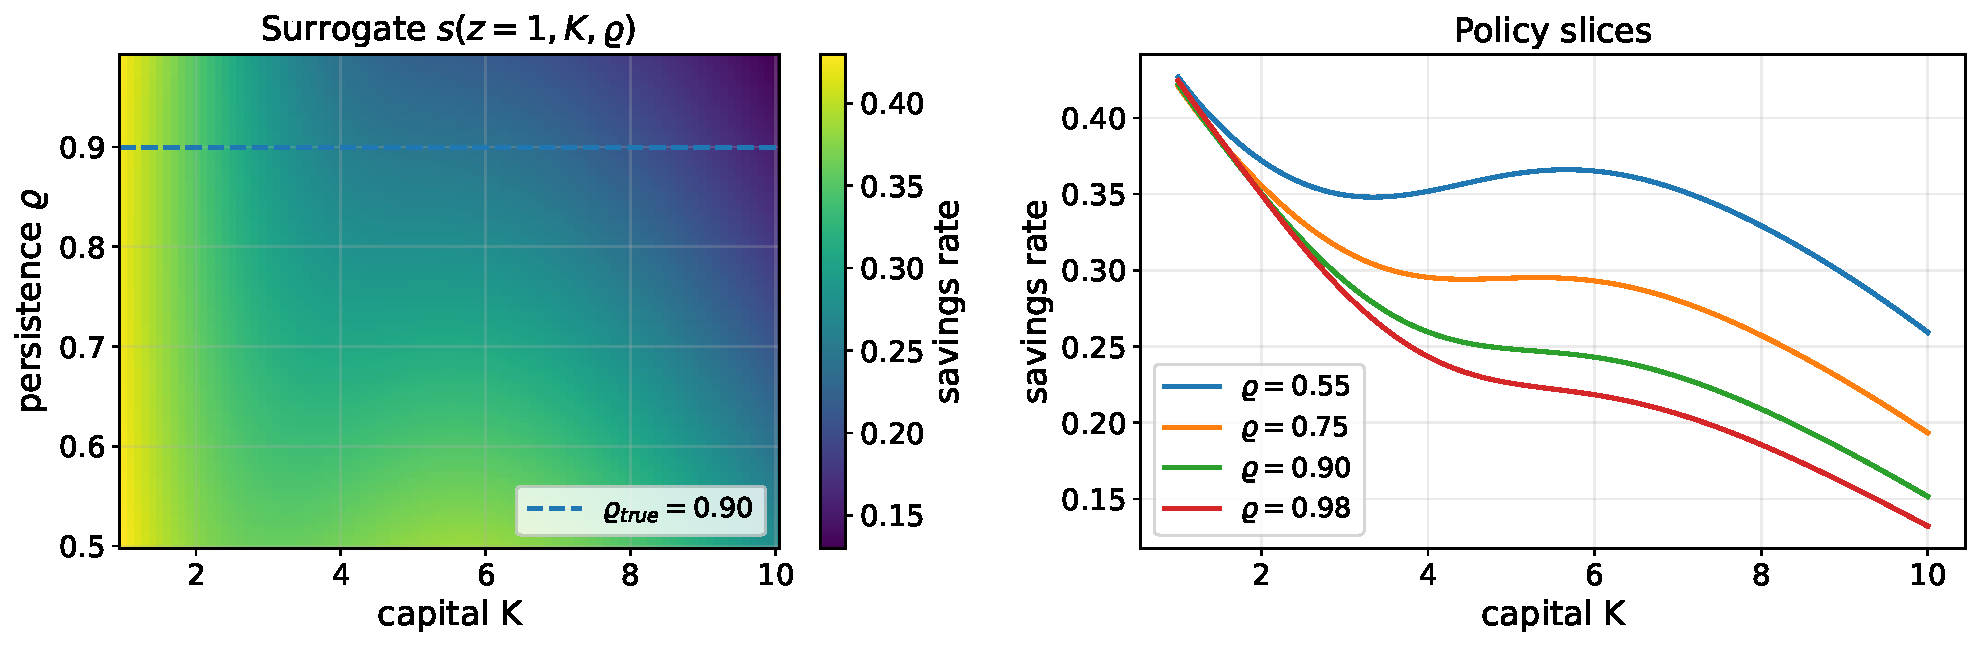
\includegraphics[width=0.94\textwidth]{figures/rho_surrogate_heatmap.pdf}
\end{center}
\vspace{-0.1cm}
{\footnotesize One trained object standing in for 99 separate model solutions. Note what it does \emph{not} show: the policy depends strongly on $K$ and only \emphc{weakly} on $\varrho$: the four slices differ by only a few per cent at low $K$, and $\varrho = 0.90$ and $0.98$ nearly coincide. That is not a defect. Most of the identifying information sits in the \emph{transition}, not the policy: $\varrho$ sets the persistence of $z$, and the moments are autocorrelations of simulated paths.}
\end{frame}

% --- Result 2 ---
\begin{frame}{Result: Which Moments Actually Identify}
\begin{center}
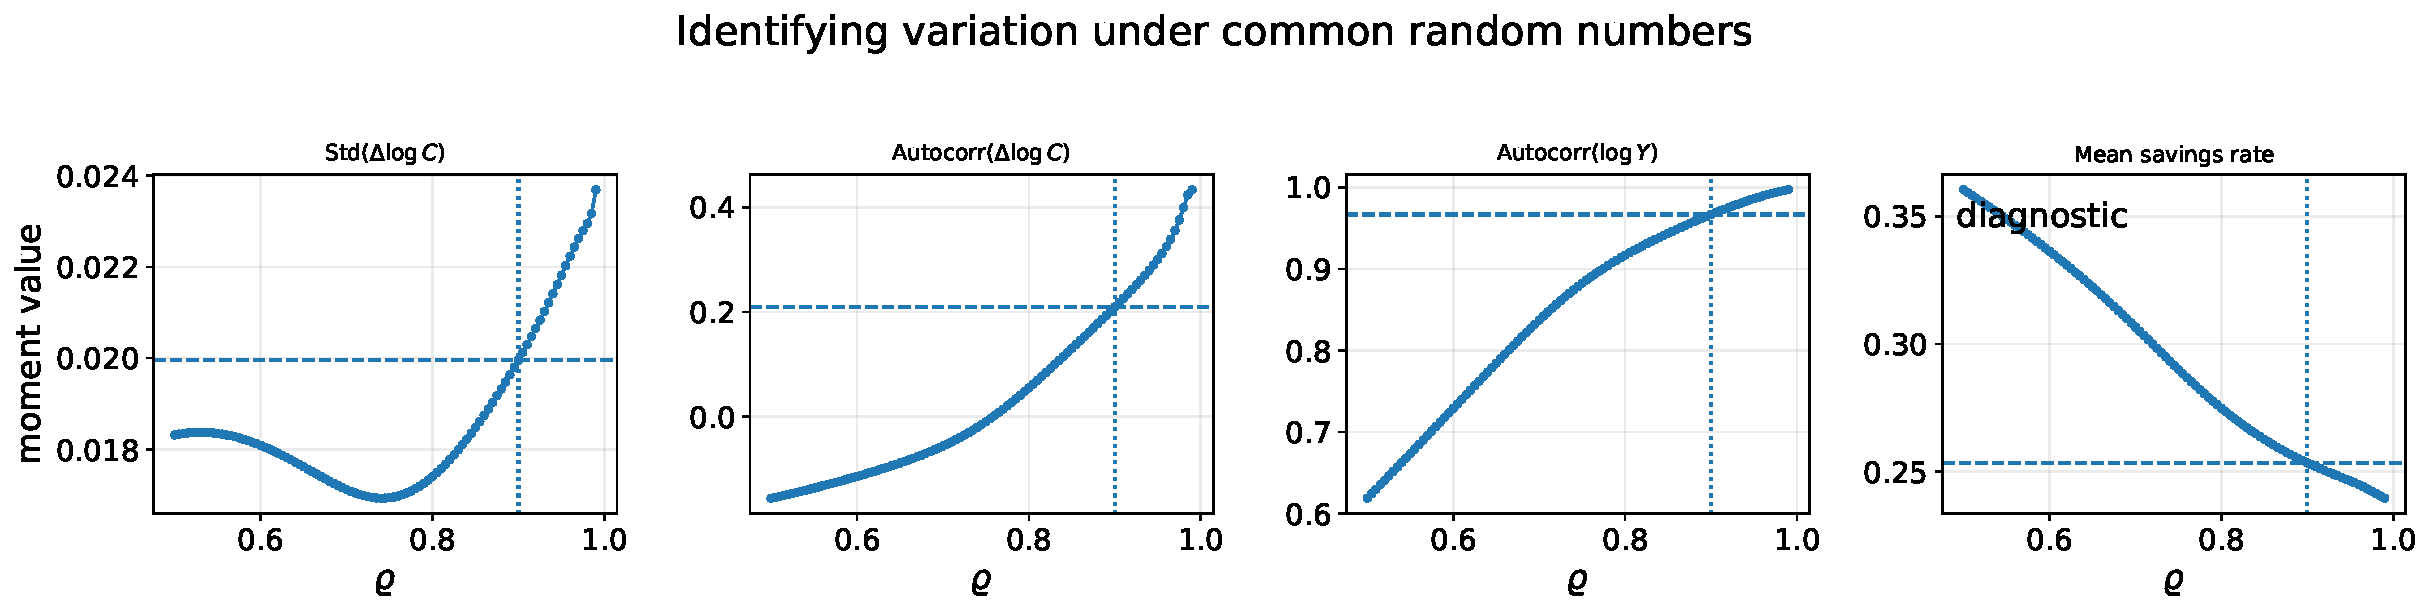
\includegraphics[width=0.96\textwidth]{figures/rho_identification.pdf}
\end{center}
\vspace{-0.1cm}
{\footnotesize $m_2$ and $m_3$ rise monotonically in $\varrho$: either alone would pin the parameter down. $m_1$ is \emphc{U-shaped}: nearly flat below $\varrho \approx 0.75$, steep above it, so it identifies well near the truth and barely at all in the lower half of the range. The diagnostic $m_0$ is \emphc{essentially flat}: its measured slope at $\varrho_{\mathrm{true}}$ is $-0.07$, against $+1.02$ for $m_2$. A moment with no slope contributes a near-zero column to $M$, and therefore almost nothing to identification, however well it matches in the data.}
\end{frame}

% --- Result 3 ---
\begin{frame}{Result: The Criterion and the Estimate}
\begin{center}
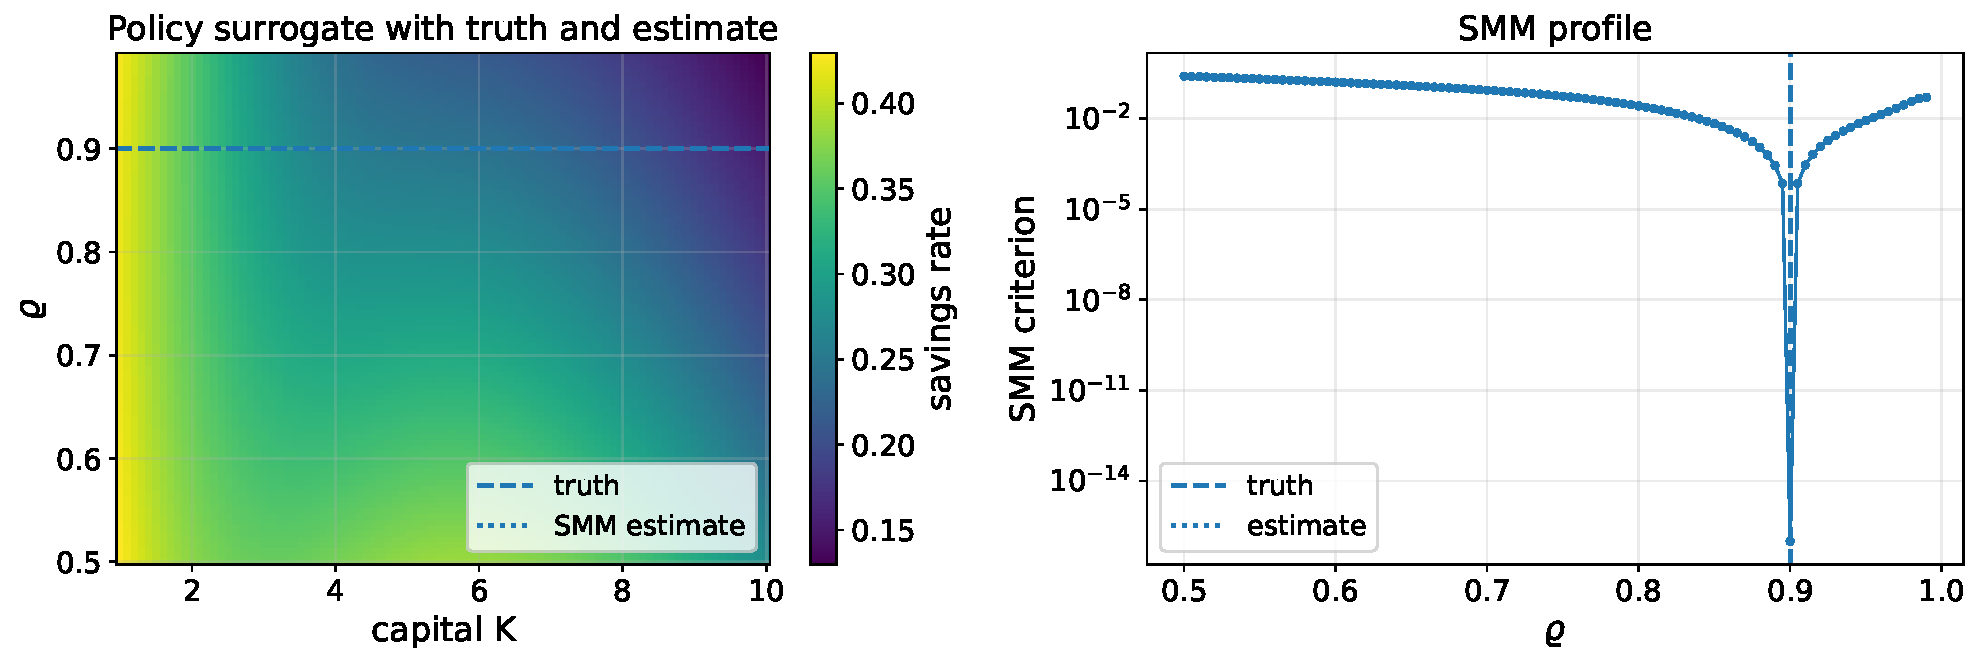
\includegraphics[width=0.94\textwidth]{figures/rho_estimate_on_surrogate.pdf}
\end{center}
\vspace{-0.1cm}
{\footnotesize A single sharp interior minimum at $\hat\varrho = \emphc{0.900}$, exact because of the design on the previous slide, not because of luck. Note the \emph{log} vertical axis: the criterion falls by three orders of magnitude between $\varrho = 0.8$ and the minimum. \emphc{Curvature this steep is what good identification looks like}, but with a zero-noise design we cannot turn it into a standard error. Contrast the next slide.}
\end{frame}

% --- Joint estimation: the ridge, and how it closes ---
\begin{frame}{Joint Estimation of $(\beta,\varrho)$: A Ridge, and How It Closes}
\begin{center}
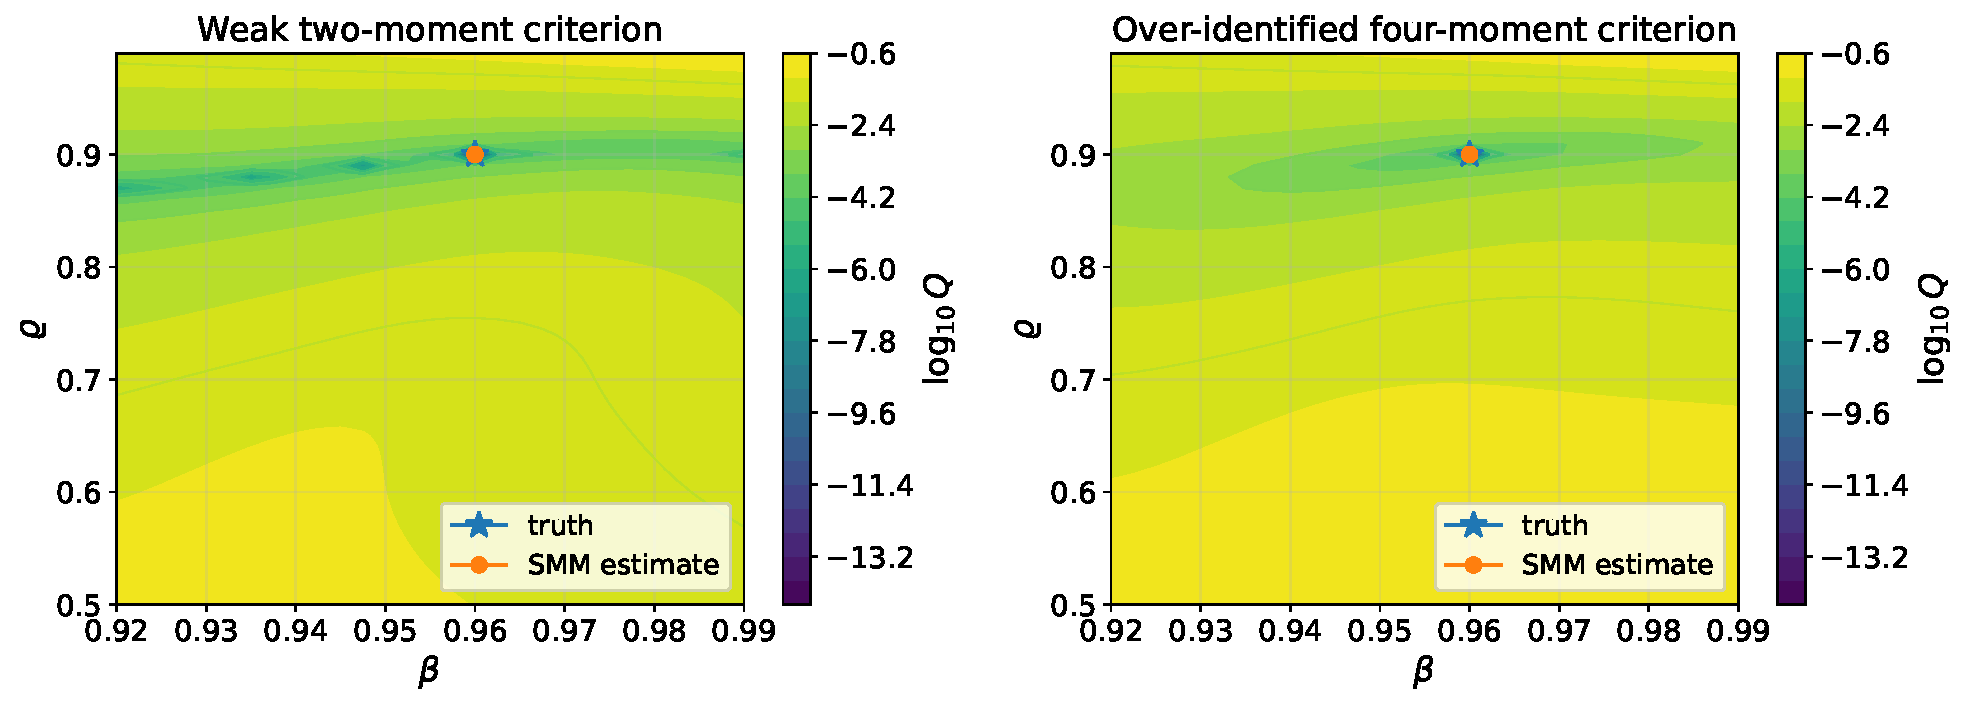
\includegraphics[width=0.94\textwidth]{figures/joint_criterion_contour.pdf}
\end{center}

\vspace{-0.25cm}
\footnotesize
\begin{columns}[T]
\column{0.48\textwidth}
\textbf{Two dynamic moments.} A long valley along $\beta$: many $(\beta,\varrho)$ pairs fit about equally well.
\emphc{Condition number 96}, smallest singular value $0.021$.
\column{0.48\textwidth}
\textbf{Add the level moments.} The valley closes into a basin.
\emphc{Condition number 2.5}, smallest singular value $0.91$.
\end{columns}

\vspace{0.15cm}
{\footnotesize The classical result: $\beta$ moves the capital stock's \emph{level}, so a level moment identifies it and business-cycle moments do not. \emphc{Identification is fixed by information, not by a better optimizer.}}
\end{frame}

% --- The ridge that wasn't ---
\begin{frame}{The Ridge That Wasn't}
\small
An earlier run of this same notebook produced a ridge that \textbf{stayed open} when the level moments were added: condition number $305$, the weak direction lying almost exactly along the $\beta$ axis. It looked like a clean econometric finding. It was not.

\vspace{0.15cm}
\begin{columns}[T]
\column{0.5\textwidth}
\begin{center}
\footnotesize
\begin{tabular}{lrr}
\toprule
& \textbf{200 steps} & \textbf{8{,}000 steps} \\
\midrule
$s$ at the anchor & $0.336$ & $0.254$ \\
error vs.\ $s^\star = 0.254$ & \emphc{$32\%$} & $0.0\%$ \\
$\partial m_0 / \partial \beta$ & \emphc{$-0.0016$} & $+1.27$ \\
condition number & $305$ & $2.5$ \\
\bottomrule
\end{tabular}
\end{center}
\column{0.46\textwidth}
The closed form gives $\mathrm{d}s^\star/\mathrm{d}\beta = 1.92$. The under-trained surrogate reported $-0.0016$: \emphc{near zero and the wrong sign}. Its Euler loss looked fine.
\end{columns}

\vspace{0.12cm}
\begin{alertblock}{The check that catches it}
A flat direction is either the moments or \emphc{the surrogate}, and the criterion cannot tell you which. Evaluate the surrogate against something known in closed form first: here $s^\star(\beta)$ at the steady state. This is \emph{lazy learning} from this morning's Part VI, caught in the act.
\end{alertblock}
\end{frame}

% --- Production ---
\begin{frame}{From Classroom to Production}
\small
Brock--Mirman is the mechanism in miniature. Chen, Didisheim \& Scheidegger (2026) run it on a high-dimensional workhorse option-pricing model.

\vspace{0.2cm}
\begin{columns}[T]
\column{0.48\textwidth}
\textbf{What the surrogate enables}
\begin{itemize}\itemsep1pt
  \item Re-estimate \emphc{every day} instead of once per paper
  \item Systematic out-of-sample evaluation against reduced-form benchmarks
  \item Conditional distributions of option returns
\end{itemize}

\column{0.48\textwidth}
\textbf{What that produced}
\begin{itemize}\itemsep1pt
  \item An option-implied \emphc{tail-risk index}, predictive of market crashes
  \item A \emphc{parameter-instability} measure that lines up with option-market illiquidity
  \item A read on the structural-versus-reduced-form trade-off
\end{itemize}
\end{columns}

\vspace{0.25cm}
\begin{alertblock}{The pattern worth remembering}
None of these are faster versions of old results. They are questions whose \emph{answers require a time series of estimates}, and that is exactly what a parametric surrogate manufactures.
\end{alertblock}
\end{frame}

% ============================================================================
% PART III: GAUSSIAN PROCESSES
% ============================================================================

% --- Padova cut: section 3 "Gaussian Processes" (651 lines) dropped ---
% --- Padova cut: section 4 "Quantify: Uncertainty" (146 lines) dropped ---
% --- Padova cut: section 5 "Design: The Optimal Carbon Tax" (257 lines) dropped ---
% --- Padova cut: section 6 "Synthesis and Hands-On" (118 lines) dropped ---
\end{document}
